\documentclass[a4paper,12pt]{article}


% add more packages if necessary
\usepackage{xspace}
\usepackage{graphicx}
%\usepackage{xcolor}
%\usepackage{hyperref}
\usepackage{amsmath}
\usepackage{subfiles}
\usepackage{float}
\usepackage{subcaption}
\usepackage{subfig}
 

% TODO: Add your group name
\newcommand{\groupname}{jcd\_dumplings\xspace}


\title{
Project Report \\ 
Group \groupname \\
\vspace{5mm}
\large Java and C\# in depth, Spring 2013
}
\author{
% TODO: Add your names here
Elmer Lukas \\
Nussbaumer Ivo
}
\date{\today}



\begin{document}
\maketitle

\section{Introduction}

This document describes the design and implementation of the \emph{Personal Virtual File System} of group \emph{\groupname}. The project is part of the course \emph{Java and C\# in depth} at ETH Zurich. The following sections describe each project phase, listing the requirements that were implemented and the design decisions taken. The last section describes a use case of using the \emph{Personal Virtual File System}.

% PART I: VFS CORE
% --------------------------------------

\section{VFS Core}

\subfile{Part1.tex}

% PART II: VFS Browser
% --------------------------------------

\section{VFS Browser}
The VFS Browser is the GUI (Graphical User Interface) for the VFS Core.
With the browser it is possible to browse through existing or new file systems and perform the usual file system actions like delete, copy, move files or folders. Furthermore it serves as a client to the synchronization server which provides the user with the possibility to synchronize the file system with the a remote server.


\subsection{Requirements}
\subsubsection{Platform}
The browser is implemented as a desktop application and is written in C\# and uses WPF (Windows Presentation Foundation).
% 1. The browser should be implemented on one of the following platforms: desktop, web or mobile.
% (a) Web applications written in C# must use Silverlight.
% (b) Web applications written in Java must either use Google Web Toolkit or JavaFX.
% (c) Mobile applications must target Android or Windows Phone.

\subsubsection{Operations}
The browser supports all operations of the VFS core.
\begin{itemize}
  \item Copy / Move / Rename / Delete
  \item Create folder
  \item Import / Export
  \item Create / Open / Close file system
\end{itemize}
% 2. The browser should support all operations from Part 1 (VFS core). For example, users should be able to select a file/folder and copy it to another location without using console commands.

\subsubsection{Selection}
Selecting a file or a folder 
Multiple selection of files or folders is possible by pressing and holding down the Control- or Shift-Key and clicking with the left mouse button or with the Up- and Down-Key.
% 3. The browser should support both single and multiple selection of files/folders.

\subsubsection{Keyboard navigation}
Most of the command are also executable by keyboard. All the other actions are accessible in the application menu, which can be opened by pressing the Alt-Key.\\
The following keyboard commands are available:\\
\\

\begin{figure}[h!]
	\centering
	\begin{tabular}{| l | l |}
		\hline
		\textbf{Command} & \textbf{Action} \\ \hline \hline
		Left / Back & Go to parent folder \\ \hline
		Right / Enter & Go to child folder / open file \\ \hline
		Up / Down & Select previous / next item \\ \hline
		Delete & Delete selected items \\ \hline
		F2 & Rename selected item \\ \hline
		Ctrl + C & Copy selected items \\ \hline
		Ctrl + X & Cut selected items \\ \hline
		Ctrl + V & Paste items \\ \hline	
	\end{tabular}
	\caption{Keyboard short cuts}
\end{figure}
% 4. The browser should support keyboard navigation. The mandatory set of operations includes folder navigation, going to parent and child folders (this is optional for mobile applications due to limited keyboard functionality).

\subsubsection{Mouse navigation}
All the commands which are accessible by keyboard are also available with mouse navigation.
Most of them are found in the application menu or the context menu of the grid. Opening a folder or a file is achieved by double clicking the item with the left mouse button and to navigate to the parent folder, the folder ".." has to be double clicked. 
% 5. The browser should support mouse navigation (or touch in case of the mobile platform). The required operations are the same as in requirement 4.

\subsubsection{Search}	
The line beneath the application menu offers all the necessary tools to search for files or folder in the file system. In the drop down menu of the split button are the following options adjustable.
\begin{figure}[h!]
	\centering
	\begin{tabular}{| l | p{10cm} |}
		\hline
		\textbf{Option} & \textbf{Description} \\ \hline \hline
		Case Sensitive & If checked, the search is case sensitive, otherwise insensitive. \\ \hline
		Global & If checked, the search is always started from the root folder, otherwise it is restricted to the current folder. \\ \hline
		Recursive & If checked, all results in the sub folders are also found, otherwise just the items in the current folder. \\ \hline
		\end{tabular}
	\caption{Search options}
\end{figure}

\begin{figure}[h!]
  \centering
  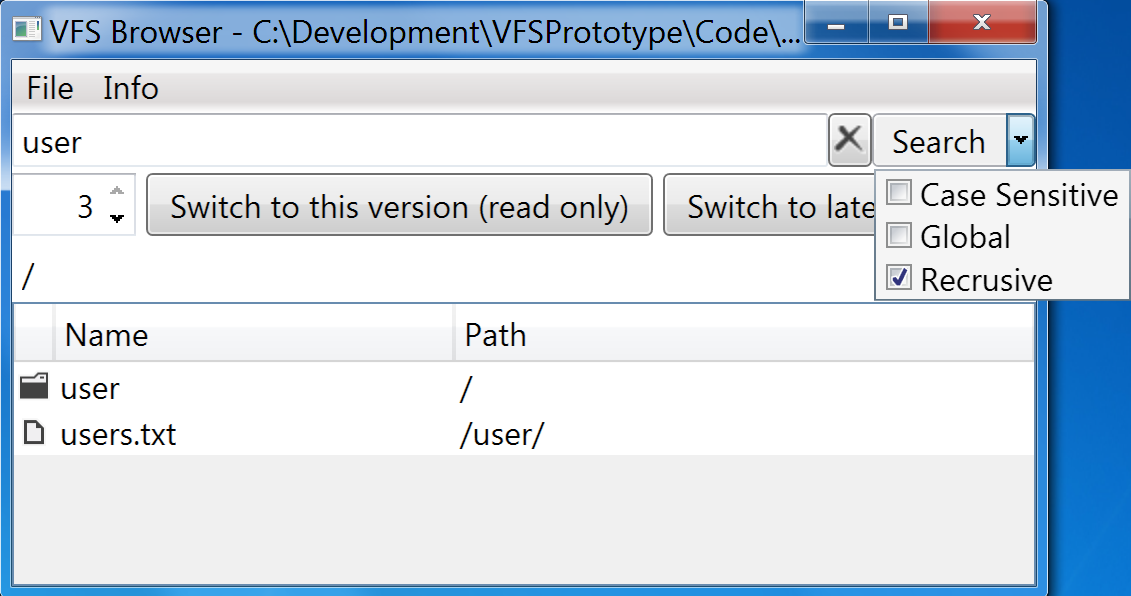
\includegraphics[scale=0.35]{Images/search.png} 
  \caption{Search functionality}
\end{figure}
% 6. The browser should support file-name search based on user-given keybwords. The search should provide options for: case sensitive/ case insensitive search; restrict search to folder; restrict search to folder and subfolders.	

\subsection{Bonus features}
\subsubsection{Responsive UI}
The VFS Browser includes a progress view, which is show during long-running operations (i.e import, copy). These operations can be cancelled by clicking the cancel button on the progress view.
\begin{figure}[h!]
  \centering
  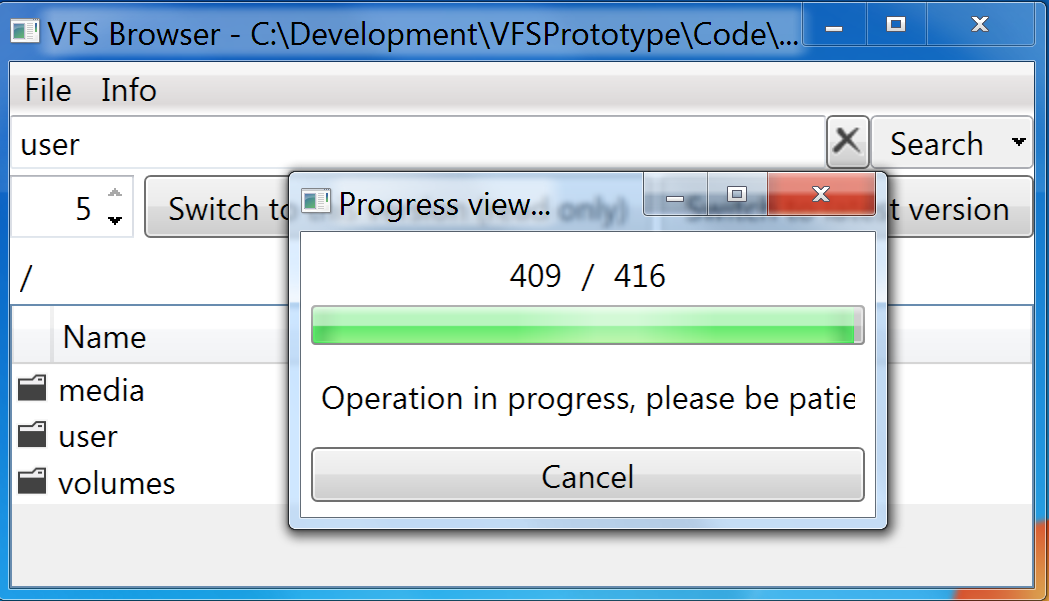
\includegraphics[scale=0.35]{Images/progress.png} 
  \caption{Progress view}
\end{figure}
% 1. Responsive UI, i.e. the browser does not stall during long-running operations (i.e. file search or import). (3p)

\subsubsection{Advanced search}
% 2. Advanced search; For example, search with wildcards/regexp, and approximate search based on some metric, e.g. edit distance. (2p)

\subsubsection{Operation progress / Drag-and-Drop}
% 3. Nice-to-have features like operation progress report (e.g. the number of files processed during export) or drag-and-drop for manipulative operations (move, copy, import). (2p)

\subsubsection{Additional Platform}
% 1. The browser is implemented for an additional platform. (5p)

\subsubsection{Efficient full-text search}
% 2. Effcient full-text search (using some sort of indexing). (4p)

% TODO: Remove this text and replace it with actual content
\emph{Describe which requirements (and possibly bonus requirements) you have implemented in this part. Give a quick description (1-2 sentences) of each requirement. List the software elements (classes and or functions) that are mainly involved in implementing each requirement.}


\subsection{Design}

% TODO: Remove this text and replace it with actual content
\emph{Give an overview of the design of this part and describe in general terms how the implementation works. You can mention design patterns used, class diagrams, definition of custom file formats, network protocols, or anything else that helps understand the implementation.}


\subsection{Integration}

% TODO: Remove this text and replace it with actual content
\emph{If you had to change the design or API of the previous part, describe the changes and the reasons for each change here.}



% PART III: Synchronization Server
% --------------------------------------

\section{Synchronization Server}

\subfile{Part3.tex}


% PART IV: Quick Start Guide
% --------------------------------------

\section{Quick Start Guide}

\subfile{Part4.tex}


\end{document}
